\documentclass[12pt,a4paper]{article}

\usepackage[margin=3cm]{geometry}

\geometry{a4paper}                   
\usepackage{setspace}
\usepackage{graphicx}
\usepackage{amsmath, amssymb}

\onehalfspacing
\setlength\parindent{0pt}

\pagestyle{empty}

\begin{document}

\begin{center}

	\large \textbf{Of queues and cures: A solution to modelling the inter time arrivals of cloud outage events}\\[12pt]

	\normalsize Jonathan Dunne$^{\ast 1}$ and David Malone$^1$ \\[12pt]
	$^1$Maynooth University (Hamilton Institute, Maynooth University, Ireland)\\ 
	$^{\ast}$Email: jonathan.dunne.2015@mumail.ie, David.Malone@nuim.ie \\[24pt]
	
\end{center}

\small \textbf{Abstract:}
The management of Cloud based outages represents a challenge for Small Medium Enterprises (SMEs), due to the variety of ways in which production outages can occur. We consider the inter-arrival times for outages events in a framework where these arrival times are used to align Systems Operations resources. Using an enterprise dataset, we address the question of how inter-arrival times are distributed by testing against a number of common distribution types. The proposed framework can help SMEs to manage their limited resource workflows. We shall also consider correlation between arrival times.

\ \*

\small \textbf{Keywords:} Distribution fitting, goodness of fit, correlation resource planning.
\vspace{-3mm}

\normalsize
\subsection*{Introduction}
For the European SME the adoption of cloud technology no easy task. Due to resource constraints and myriad of failure patterns, SMEs face challenges in providing a reliable and stable service platform for their customer's needs. In this paper we describe a framework, that the SME an leverage to best manage their limited set of resources as part of incoming outage events in their cloud infrastructure. 

\subsection*{Data Set}
The study presented in this paper examines approximately 250 cloud outage events from a large enterprise system. Our study aims to answer a key question: Which distribution is best suited to model the interarrival time of cloud outage events. To answer this question a number of common distribution types were modelled; lognormal, gamma, Weibull, exponential, logistic, loglogistic and Pareto.
\par

\subsection*{Results}
Each distribution was modelled against the interarrival times of the dataset using the R computer package and the fitdistrplus library which also calculates the distribution parameters. Using a second package ADGofTest, the parameters of each distribution validated for their goodness of fit. Table 1 summarises the results of this test.

\begin{table}[!ht]\centering
\caption{\label{myname_uni:tab1} Summary of Anderson-Darling GoF statistics.}
% A table with three columns, where e.g. the first is left aligned,
% the second has centred entries, and the third is right aligned
\begin{tabular}{lcr}
Distribution Name  & AD statistic & p-value \\
\hline
lognormal  & 3.039  & 0.026  \\
gamma  & 6.034  & 9.347e-04  \\ 
Weibull   & 0.975 & 0.371 \\
exponential  & 3.110  & 0.024 \\
logistic  & 12.819 & 2.765e-06  \\
loglogistic  & 1.823  & 0.115 \\
Pareto  & 0.661  & 0.592 \\
\end{tabular}
\end{table}

%% Uncomment the figure environment below to include graphics %%
\begin{figure}[ht!]\centering
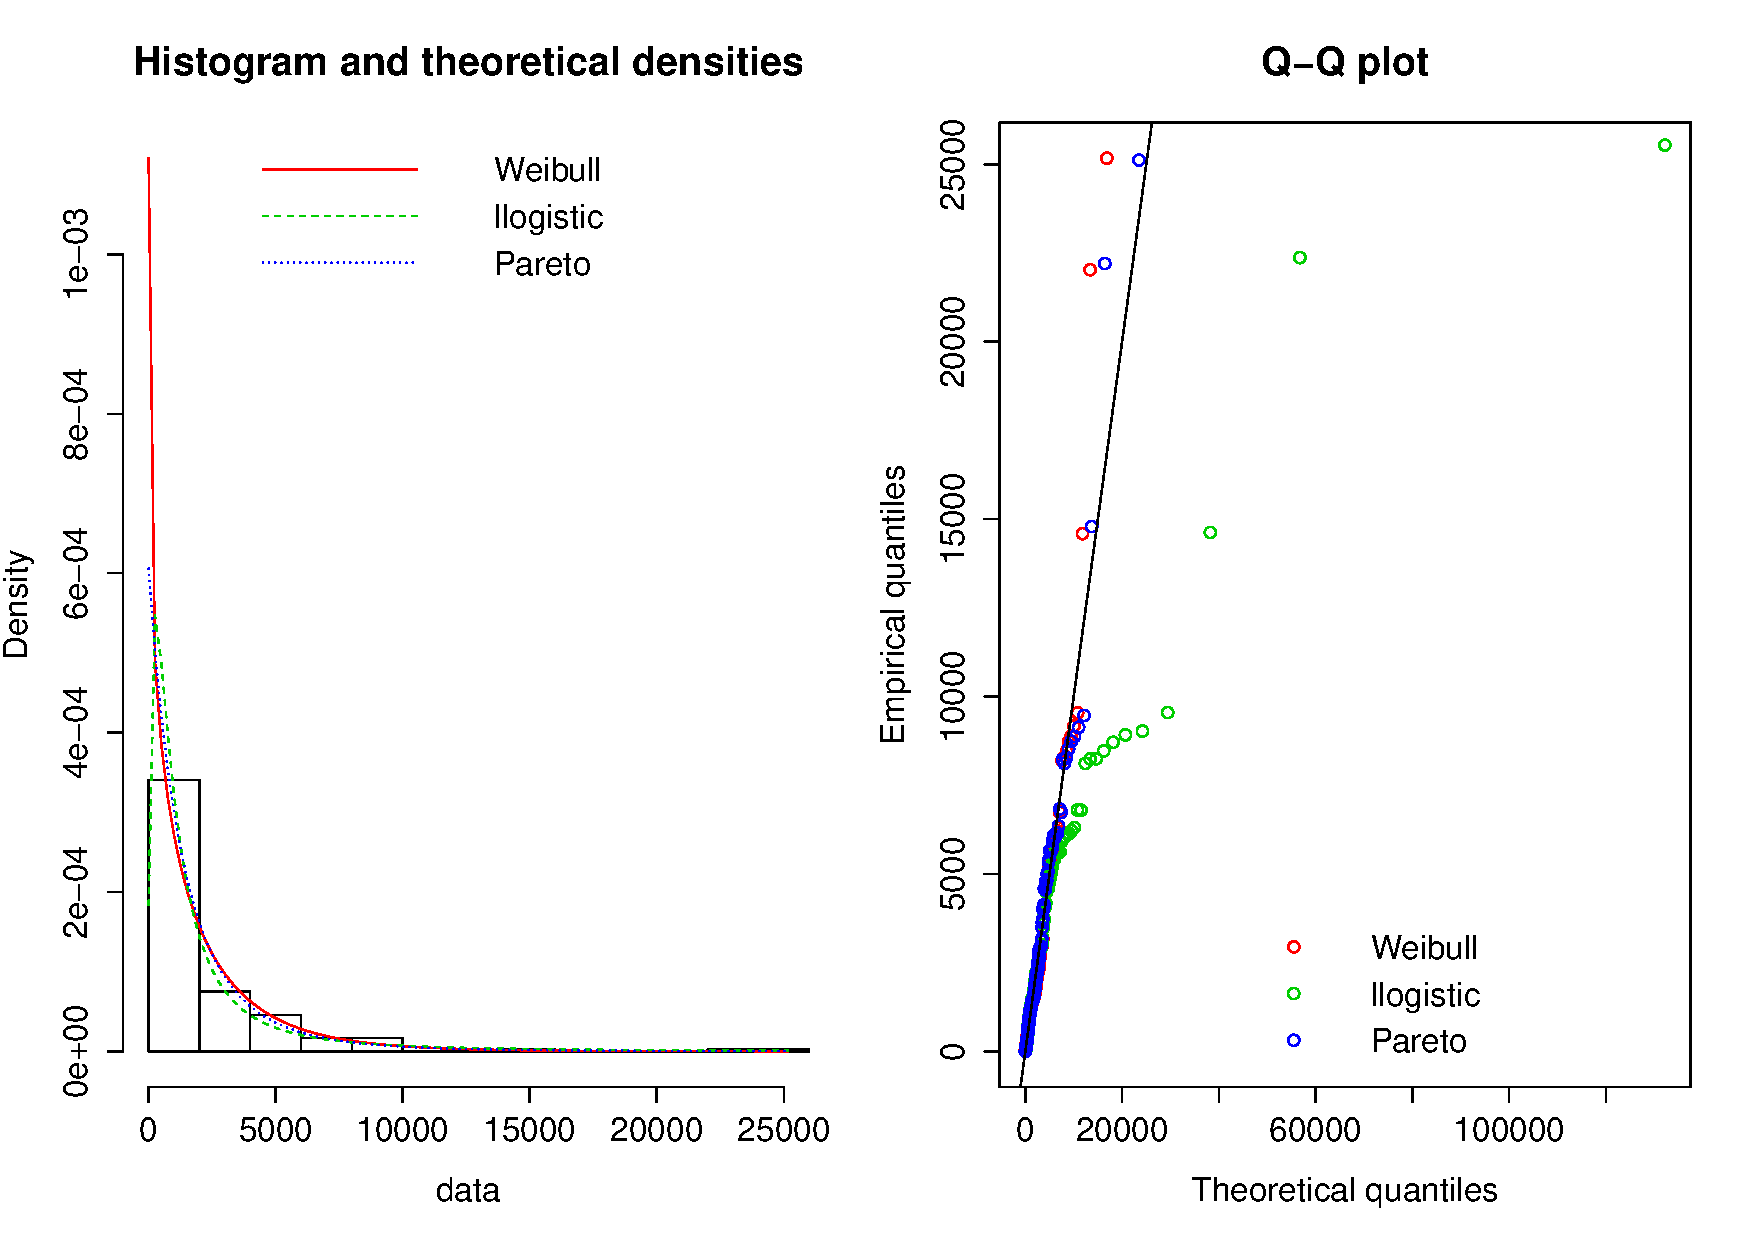
\includegraphics[width=7.4cm, height=5cm]{Graphs1.pdf}
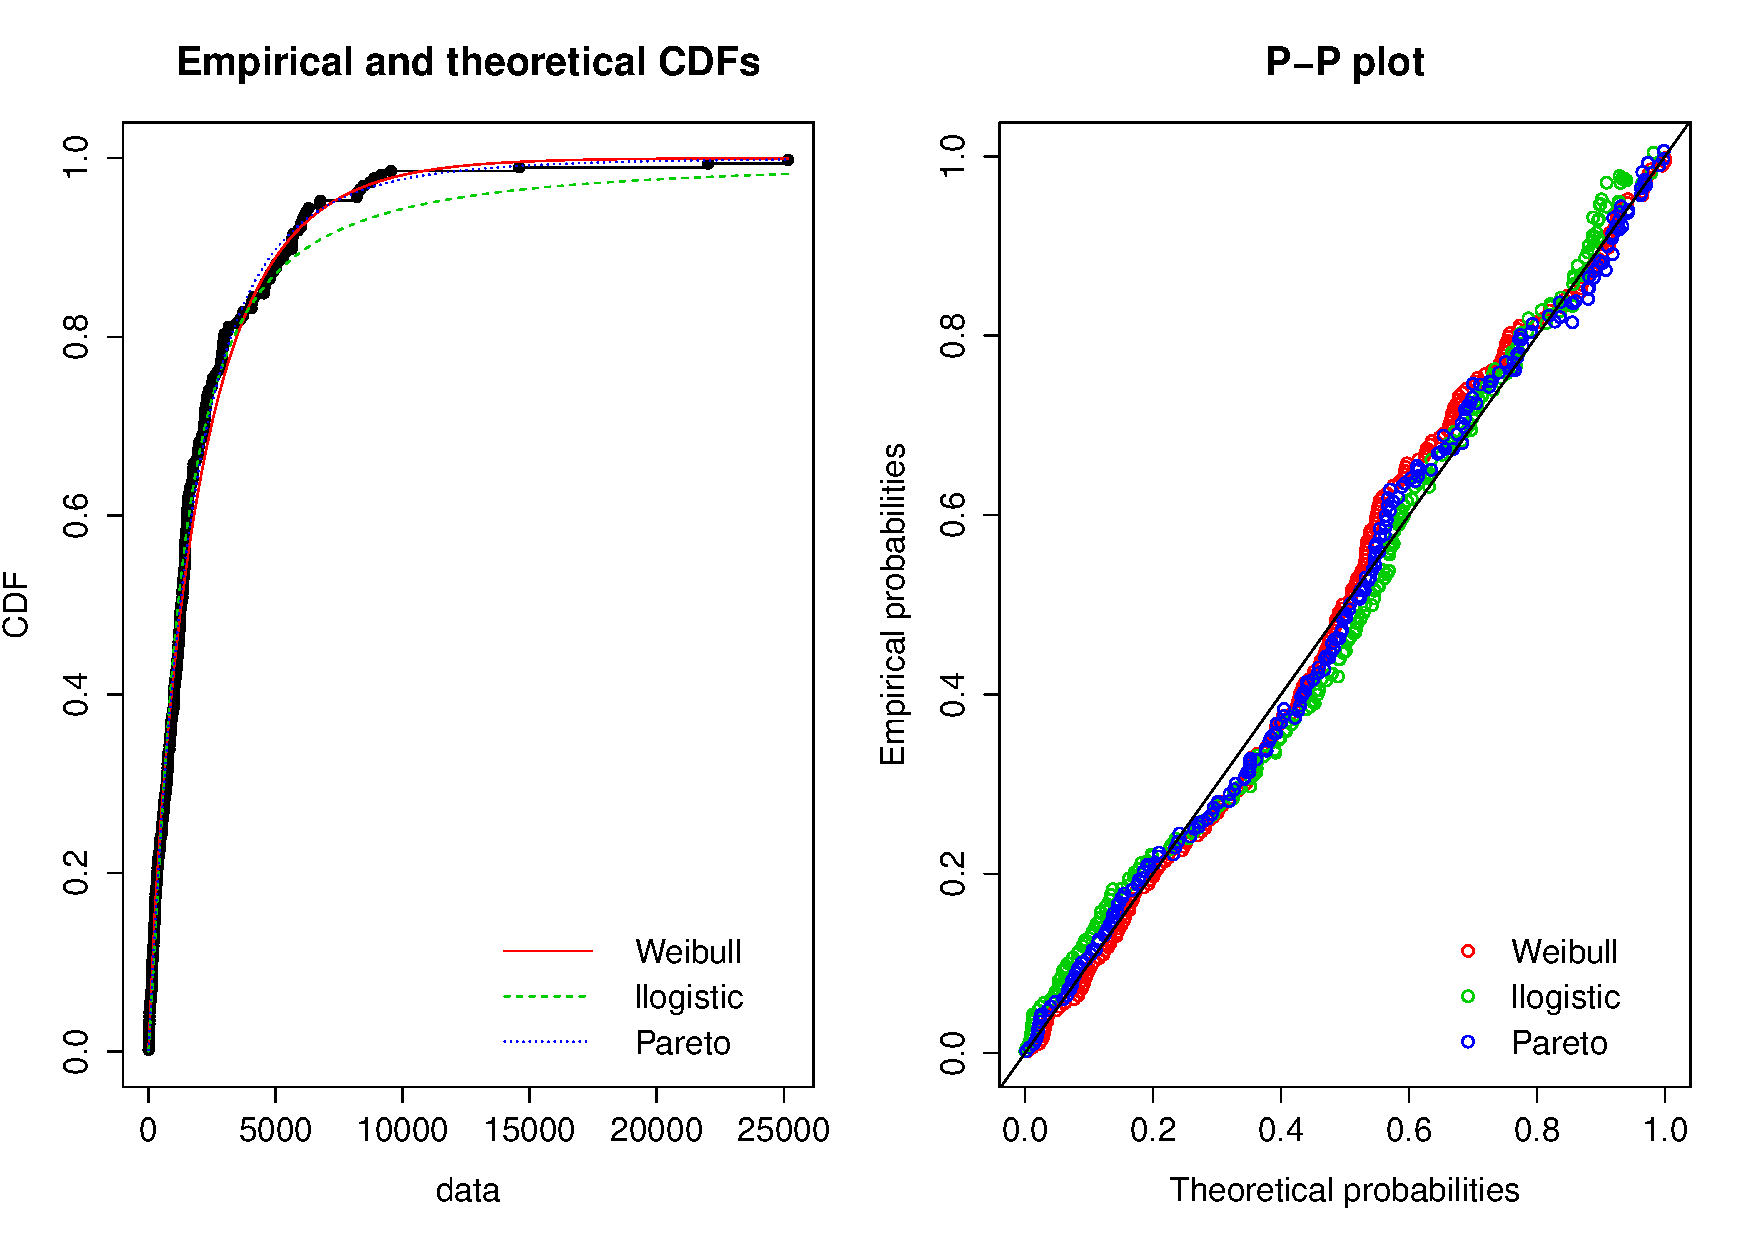
\includegraphics[width=7.4cm, height=5cm]{Graphs2.pdf}
\caption{\label{myname_uni:fig1} Four goodness-of-fit plots for Weibull, loglogistic and Pareto distributions fitted to the interarrival times from the cloud outage data set.}
\end{figure}

\vspace{-8mm}

\subsection*{Discussion}
Table 1 shows that Pareto has the best p-value for the Anderson-Darling test, followed by loglogistic and Weibull. All other distributions were rejected as part of hypothesis testing. Figure 1 shows goodness of fit plots for the three best fitted distributions. The quantile-qualtile plot shows that the Pareto distribution more closely models the data set even for extreme values.


\subsection*{Conclusion}

It was found that the Pareto distribution is a useful distribution for modelling the interarrival times of cloud outages. This result can be used by SMEs as an arrival time parameter for a queuing model for cloud outage events. 

\subsection*{References}
\small
% Ensure font of references section is small
\begin{description}
\item[Delignette-Muller, M.L. and Dutang, C. and Pouillot, R. and Denis, J.B.] (2015). 
	Web Page https://cran.r-project.org/web/packages/fitdistrplus/index.html
\item[Bellosta, C.J.G] (2011).
	https://cran.r-project.org/web/packages/ADGofTest/index.html
\end{description}
\end{document}








